% !TEX root = ModelRisk_spring14UDE.tex

\part{A Theory of Model Risk}

\section{What is Model Risk?}

% frametitle
{SST Classification of Risk Types}
\begin{figure}
	\centering
		\includegraphics[width=0.8\textwidth]{../../../pics/risk_SST}
	\label{fig:Risk_map1}
\end{figure}

% frametitle
{Deutsche Bank Risk Types}
\begin{figure}
	\centering
		\includegraphics[width=0.8\textwidth]{../../../pics/DeutscheBank-RiskTypes}
	\label{fig:Risk_map2}
\end{figure}

% frametitle
{Deutsche Bank Annual Report 2012}
\begin{itemize}
\item<1->
Credit risk, market risk and operational risk attract regulatory capital.
\item<2-> Liquidity risk is the risk arising from our potential inability to meet all payment obligations when they come due or only being able to meet these obligations at excessive costs.
\item<3->Business risk describes the risk we assume due to potential changes in general business conditions, such as our market environment, client behavior and technological progress.
\item<4->Reputational risk is the risk that publicity concerning a transaction, counterparty or business practice involving a client will negatively impact the public's trust in our organization.
\item<5->Furthermore, they mention Insurance specific risk and risk concentration.
\end{itemize}

% frametitle
{Basel Regulation I}
Regulators formulate some principles for models
\begin{itemize}
\item<1-> Uncertainty is specific to the instrument and the point in time the valuation is effected.
\item<2-> A bank is expected to consider all relevant market information likely to have a material effect on an instrument's fair value when selecting the appropriate inputs.
\item<3->Observable inputs or transactions may not be relevant. In such cases, the observable data should be considered, but   may not be determinative.
\end{itemize}

% frametitle
{Basel Regulation II}
\begin{itemize}

\item<1-> There are also operative recommendations
\begin{itemize}
\item Validation includes evaluation of the model's theoretical soundness and mathematical integrity and the appropriateness of model assumptions, including consistency with the market.
\item A bank should use a range of approaches and cross-check validations.
\item Valuation models should be tested and reviewed under possible stress conditions. There should be defined triggers for such reviews.
\end{itemize}

\item<2->
Basel III introduces a risk-invariant leverage ratio of 3 percent in recognition that models may be biased.

\end{itemize}

% frametitle
{Motivation}
\begin{itemize}
\item<1-> Model risk has been recognized as one of the fundamental reasons for financial distress for banks and insurance companies.
Recently, a number of authors addressed this issue:
\begin{itemize}
\item Schoutens et. al. (2004): A perfect calibration - now what?
\item Cont (2006): Model uncertainty and its impact on the pricing of derivative instruments.
\item Bann{\"o}r, Scherer (2011): Quantifying the degree of parameter uncertainty in complex stochastic models
\item Morini, M. (2011): Understanding and Managing Model Risk, Wiley.
\end{itemize}
\item<2-> Important questions:
\begin{itemize}
\item How sensitive is the value of a given derivative to the choice of the pricing model (parametric setting)?
\item Can one quantify a provision for model risk (as for market and credit risk)?
\end{itemize}

\end{itemize}

% frametitle
{Schoutens - CallFit, NIGCIR}
\begin{figure}[htp]
\centering
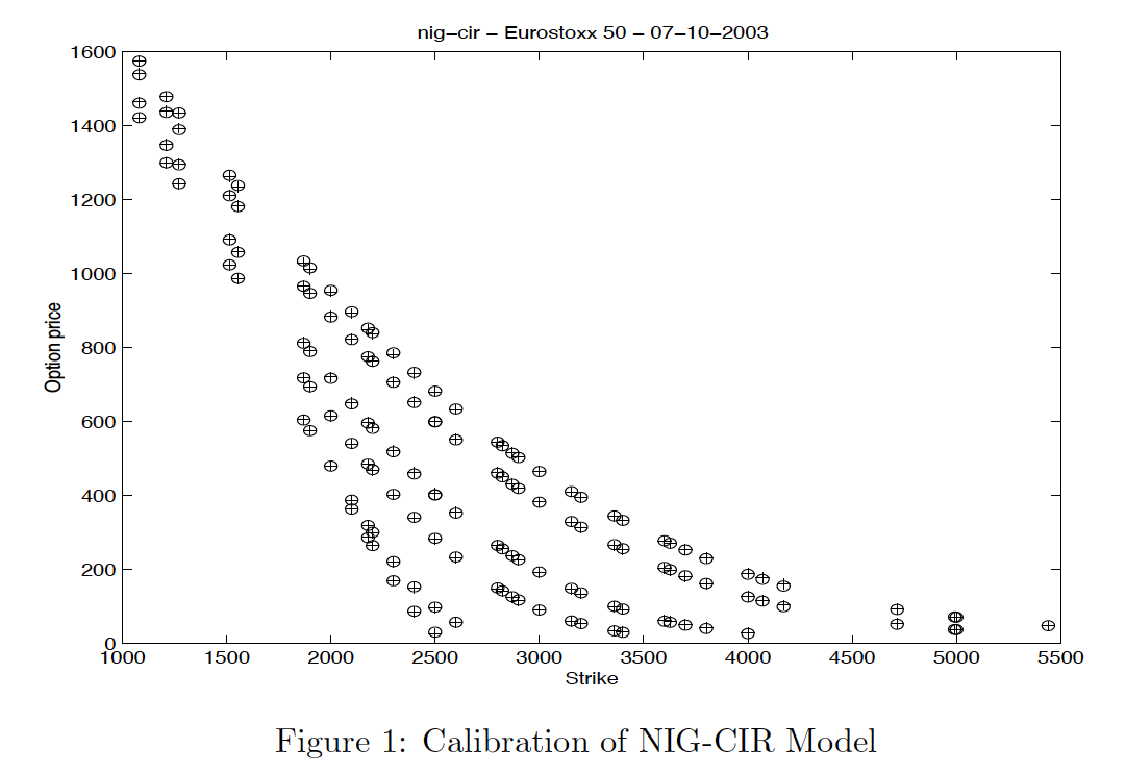
\includegraphics[width=\textwidth]{../../../pics/WS-CallFit.pdf}
\end{figure}

% frametitle
{Schoutens - CallFit, BNS}
\begin{figure}[htp]
\centering
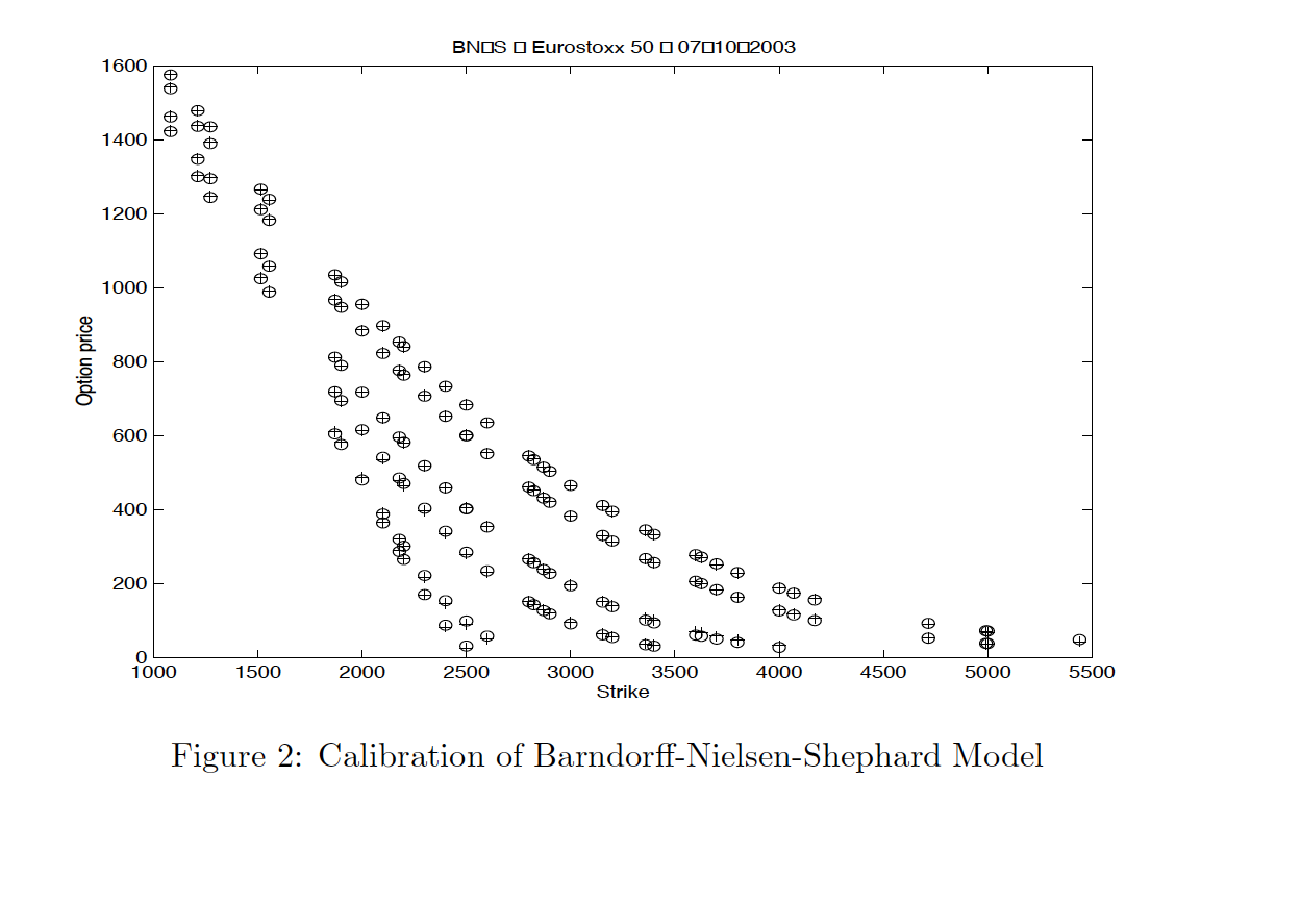
\includegraphics[width=\textwidth]{../../../pics/WS-CallFitBNS.pdf}
\end{figure}

% frametitle
{Schoutens - Exotic Fit}
\begin{figure}[htp]
\centering
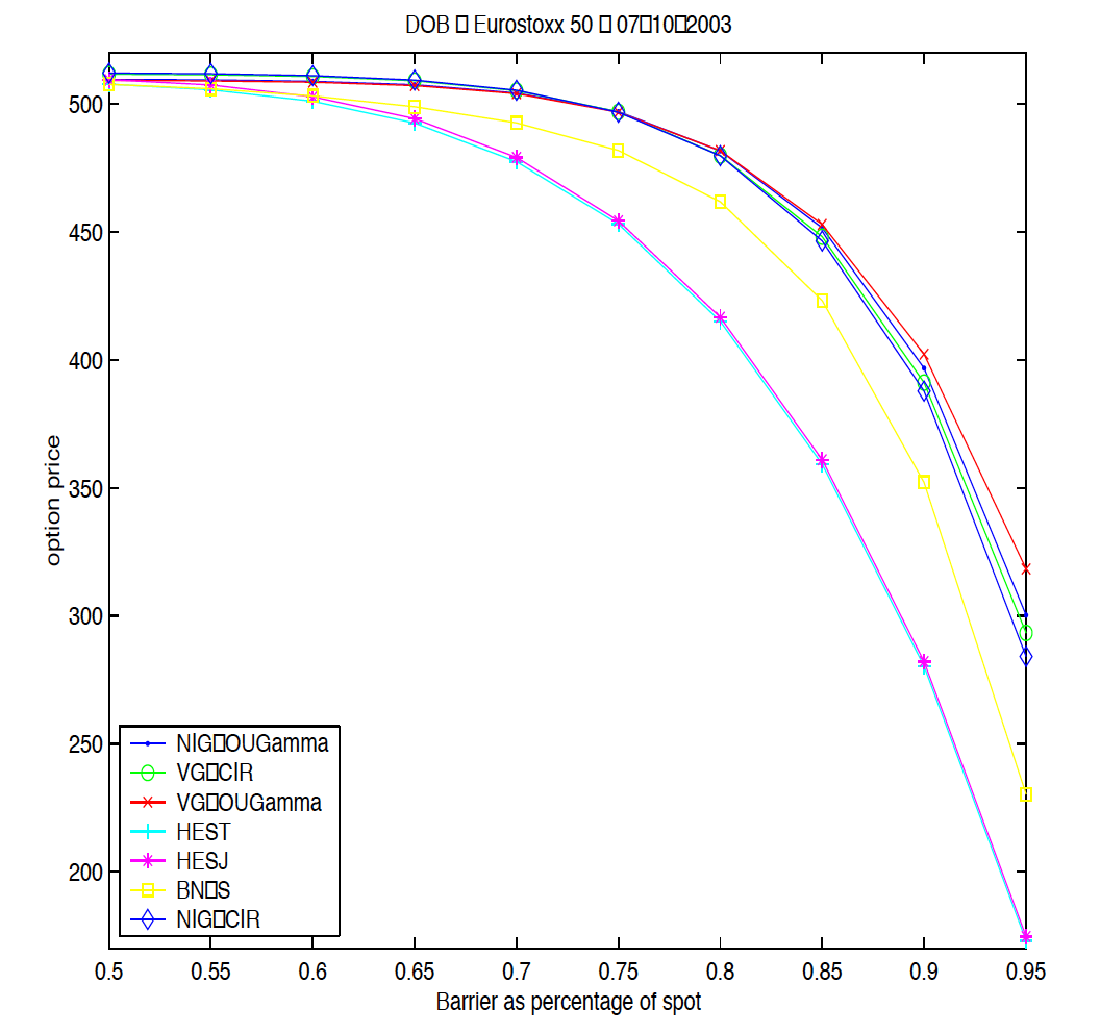
\includegraphics[width=0.7\textwidth, heigth=0.5\textheigth]{../../../pics/WS-ExoticFit.pdf}
\end{figure}

% frametitle
{Schoutens - Clique Fit}
\begin{figure}[htp]
\centering
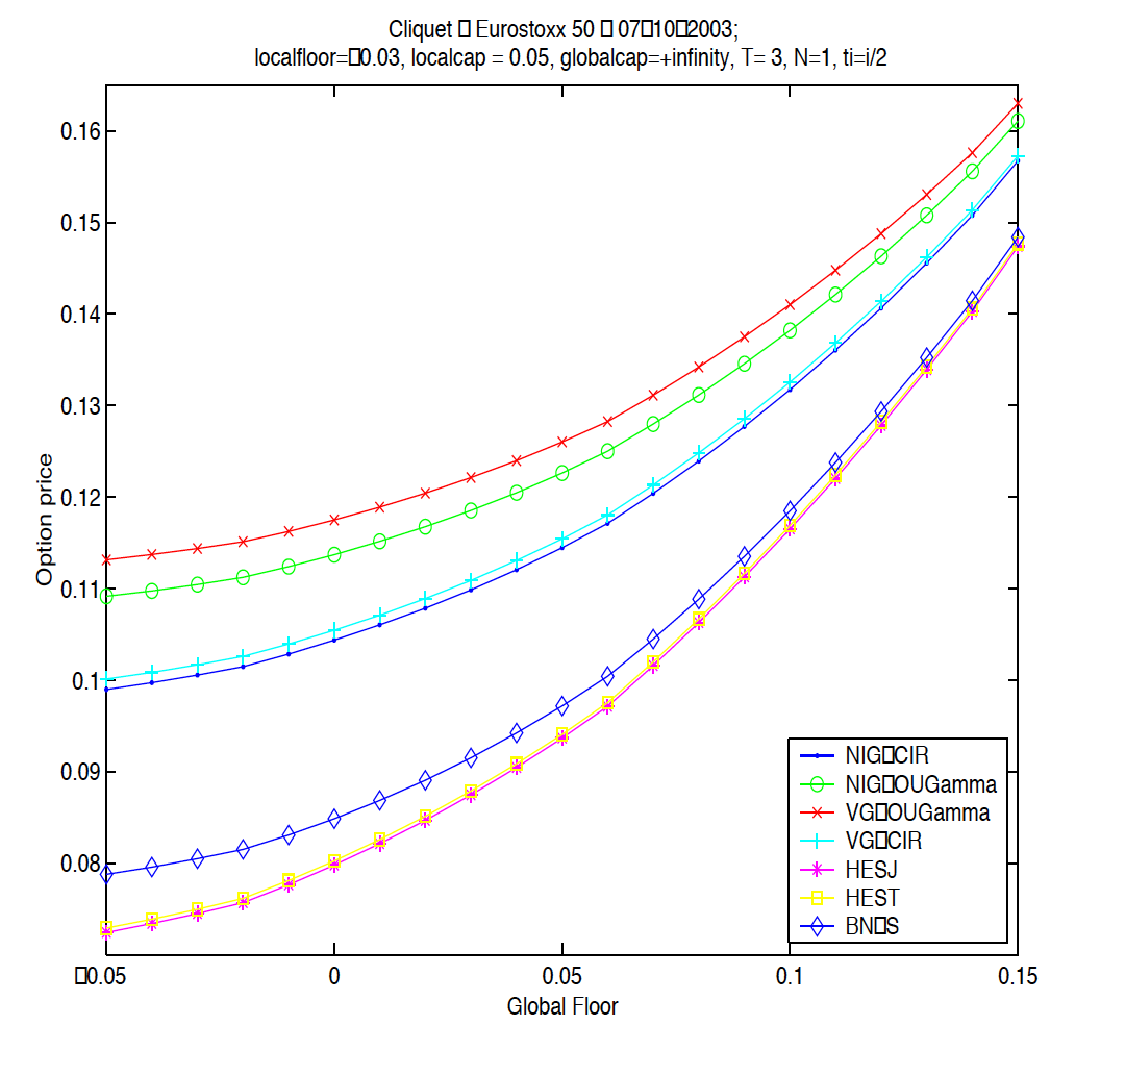
\includegraphics[width=0.7\textwidth, heigth=0.5\textheigth]{../../../pics/WS-CliqueFit.pdf}
\end{figure}

% frametitle
{How to define model risk?}
\begin{itemize}
\item {\it Simple Idea:} Model risk is the possibility that a (financial) institution suffers losses due to mistakes in the development and application of (validation) models.
\end{itemize}

% frametitle
{Derman (1996) -- Value Approach}
\begin{itemize}
\item Is the payoff accurately described?
\item Is the software reliable?
\item Has the model been appropriately calibrated to the prices of the simpler, liquid constituents that comprise the derivative?
\item Does the model provide a realistic description of the factors that affect the derivative's value?
\end{itemize}
Last point: Residual risk relating to the factors -- model risk?

% frametitle
{Rebonato (2003) -- Price Approach}

\begin{itemize}
\item<1-> Model risk is the risk of occurrence of a significant difference between the mark-to-model value of a complex and/or illiquid instrument and the price at which the same instrument is revealed to have traded in the market.
\item<2-> Thus, models can be counterintuitive, unreasonable, maybe not even free of arbitrage, as long as the market agrees with the valuation.
\item<3-> So, large losses  can only happen when a sudden gap opens between market prices and model valuation.
\end{itemize}

% frametitle
{J. Hull: Risk Management and Financial Institutions}
For pricing models are used to
\begin{itemize}
\item<1-> observe model prices for similar instruments that trade
\item<2-> imply model parameters and interpolate as appropriate
\item<3-> value new instrument
\item<4-> perform reverse engineering from prices observed from counterparty quotes to understand their models
\end{itemize}
Model Risk can lead to ..
\begin{itemize}
\item<1->
Incorrect price at time product is bought or sold
\item<2-> Incorrect hedging
\end{itemize}

% frametitle
{Marking Prices of an Instrument to Market}
\begin{itemize}
\item<1->
Use price quoted by market maker (usually financial institutions mark to mid of bid and offer)
\item<2-> Use price at which financial institution has traded product
\item<3-> Use interdealer broker prices
\item<4-> Use interdealer price indications
\item<5-> Use model (marking to model)
\item<6-> Contact member of the trading community
\end{itemize}

% frametitle
{Products}
\begin{itemize}
\item<1-> Linear products: Very little uncertainty about the right model, but mistakes do happen
\item<2-> Standard Products
\begin{itemize}
\item We do not need usually a model to know the price of an actively traded product. The market tells us the price.
\item The model is a communication tool (e.g., implied volatilities are quoted for options)
\item It is also an interpolation tool (e.g., a tool for interpolating between strike prices and maturities)
\end{itemize}
\item<3-> Non-Standard Products
\begin{itemize}
\item In the case of nonstandard products models play a key role in both pricing and hedging
\item It is a good idea to use more that one model whenever possible
\end{itemize}
\end{itemize}

% frametitle
{Hull: Model Risk}
\begin{itemize}
\item<1->  Dangers in Model Building
\begin{itemize}
\item Overfitting
\item Overparametrization
\end{itemize}
\item<2-> Detecting Model Problems
\begin{itemize}
\item<1-> Monitor types of trading a financial institution is doing with other financial institutions
\item<2-> Monitor profits being recorded from trading of different products (over- reap. under-pricing).
\item<3-> Use Model Audit Group
\begin{itemize}
\item Check that a model has been implemented correctly
\item Examine whether there is a sound rationale for the model
\item Compare the model with others that can accomplish the same task
\item Specify limitations of model
\item Assess uncertainties in prices and hedge parameters given by model
\end{itemize}
\end{itemize}
\end{itemize}

\section{Tools to Assess Model Risk}
\subsection{Risk, Uncertainty, and Ambiguity}

% frametitle
{Definitions}
\begin{itemize}
\item<1-> Typically a stochastic model $(\Omega, \F)$ defining future scenarios and a
probability measure $\prob$ on these outcomes.
\item<2->  We have to distinguish between
\begin{itemize}
\item {\it Risk:}  we are able to specify a unique $\prob$
\item {\it (Knightian) Uncertainty:} we are not able to specify a precise $\prob$
\item {\it Ambiguity:}  we are facing several possible specifications $\prob_1, \prob_2, \ldots$\end{itemize}
\item<3-> Approaches to deal with ambiguity are "averaging" and "worst-case".
\end{itemize}

% frametitle
{Bayesian Model Averaging}
\begin{itemize}
\item<1-> Let ${\cal M}= \{M_1, \dots, M_J\}$ be a family of models and  $\{\Theta_1, \dots, \Theta_J\}$ the corresponding parameter spaces.
\item<2->  A Bayesian observer has
\begin{itemize}
\item a prior on model parameters $p(\theta_j|M_j)$
\item a prior on model weights $\prob(M_j)$
\end{itemize}
\item<3-> Given a set of observations $y$ the posterior probabilities are
$$
\prob(M_j|y) = \frac{p(y|M_j)\prob(M_j)}{\sum_{k=1}^{J}p(y|M_k)\prob(M_k)}
$$
with
$$
p(y|M_j)=\int_{\Theta_j} \prob(y|\theta_j, M_j)p(\theta_j|M_j) d\theta_j.
$$
\end{itemize}

% frametitle
{Bayesian Model Averaging -- Valuation}
\begin{itemize}
\item<1-> If we want to compute a model dependent quantity $X$ given by an expectation we average over models.
\item<2-> Given a set of observations $y$ the posterior expectation is
$$
\EX(X|y) = \sum_{j=1}^{J} \EX(X |y, M_j) \prob(M_j |y).
$$
\item<3-> Problems:
\begin{itemize}
\item how to specify priors (stock vol vs jump diffusion?)
\item computational intensive
\end{itemize}

\end{itemize}

% frametitle
{Worst-Case Approach}
\begin{itemize}
\item<1-> The worst-case approach has its foundations in the "MaxMin" approach as a robust version of expected utility. \item<2-> Assume $U$ is a utility function, then
$$
\max _X \min_{\prob \in {\cal P}} \EX_{\prob}(U(X)).
$$
\item<3-> Separation of risk-aversion and aversion to ambiguity
\begin{itemize}
\item risk aversion is captured in $U$
\item aversion to ambiguity is captured in $\min$
\end{itemize}

\end{itemize}

\subsection{Risk Measures}

% frametitle
{Convex Risk Measures}

Let $(\Omega, \F)$ be a measurable space and ${\cal X} \subset {\cal L}^0(\Omega)$ a vector space. ${\cal Y} \subset {\cal X}$ be a sub-vector space and
$\pi \in {\cal Y}^*$.
\begin{equation}
\rho: {\cal X} \rightarrow \setR
\end{equation}
is a convex risk measure with $\pi$ translation invariance iff
\begin{itemize}
\item $\rho$ is monotone: $$X \leq Y \;  \implies \; \rho(X) \geq \rho(Y).$$
\item $\rho$ is convex: $$\forall \lambda \in [0,1]: \rho(\lambda X + (1-\lambda) Y) \leq \lambda \rho(X) + (1-\lambda) \rho(Y).$$
\item $\rho$ is $\pi$-translation invariant: $$\forall Y \in {\cal Y}: \rho(X+Y) = \rho(X) + \pi(Y).$$
\end{itemize}

% frametitle
{Coherent Risk Measures}

A coherent risk measure is a function $\rho$ on abstract risk positions such that
\begin{itemize}
\item<1-> \emph{Monotonicity}: if $X\geq 0$, then $\rho(X)\leq 0$;
\item<2-> \emph{Translation invariance}: if $k \in \R$, then
$\rho(X+k)=\rho(X)-k$;
\item<3-> \emph{Homogeneity}: if $\lambda \geq 0$ in $\R$, then $\rho(\lambda X)
= \lambda \rho (X)$;
\item<4-> \emph{Subadditivity}: $\rho(X+Y)\leq \rho(X)+\rho(Y)$.
\end{itemize}

% frametitle
{Convex Risk Measures -- Properties}

\begin{itemize}
\item $\rho$ is coherent $\Leftrightarrow \; \rho(cX) = c \rho(X), \; \forall c>0$.
\item $\rho$ is normalized $\Leftrightarrow \; \rho(0) = 0$.
\item Let $\prb$ be a probability measure on $(\Omega, \F)$.\\
$\rho$ is $\prb$-law invariant $\Leftrightarrow \; \prb^X = \prb^Y $ implies $\rho(X) = \rho(Y)$.
\end{itemize}

% frametitle
{Examples: VaR and AVaR}
\begin{itemize}
\item general probability space $(\Omega, \F, \prb)$, $\beta \in (0,1]$, $X\in L^1(\prb)$, then
$$
VaR_\beta(X) = q_{-X}^{\prb}(1-\beta).
$$
 \item VaR is not a coherent risk measure as it is not subadditive in general.
\item the average value at risk at level $\alpha \in (0,1]$ is
$$
AVaR_\alpha(X) = \frac{1}{\alpha} \int_0^\alpha VaR_\beta(X) d\beta.
$$
\item AVaR$_\alpha$ is a convex risk measure (coherent and law-invariant).
\end{itemize}

% frametitle
{Value at Risk}
The worst $1-\alpha$ scenarios are below the $-VaR_\alpha$, all others are below.
\begin{figure}
	\centering
		\includegraphics[width=0.8\textwidth]{../../../pics/VaR}
	\label{fig:VaR}
\end{figure}

% frametitle
{Value at Risk}
The figure illustrates a portfolio with a low VaR compared to its risk.
\begin{figure}
	\centering
		\includegraphics[width=0.7\textwidth]{../../../pics/Shortcoming_VaR}
	\label{fig:Shortcoming_VaR}
\end{figure}

% frametitle
{Average Value-at-Risk (AVaR) }
\begin{itemize}
\item<1-> The AVaR specifies the expectation of the loss in case the loss is above the VaR.
\item<2-> AVaR is also called Tail Value-at-Risk (TVaR) or Conditional
Value-at-Risk (CVaR) or  Expected Shortfall (ES).
\end{itemize}

% frametitle
{Illustration of AVaR}
\begin{figure}
	\centering
		\includegraphics[width=1\textwidth]{../../../pics/Expected_Shortfall}
	\label{fig:Expected_Shortfall}
\end{figure}

\section{Stochastic Models of Financial Markets}
\subsection{Model Setting}

% frametitle
{ Financial Market Model}
\begin{itemize}
\item<1->
$T>0$ is a fixed a planning horizon.
\item<2->
Uncertainty in the financial market is modelled by a probability
space $(\Omega, {\cal F},\prb)$ and an information set  (filtration) $\fil =({\cal
F}_t)_{0\leq t\leq T}$.
\item<3->
There are $d+1$ primary traded assets, whose price processes are
given by stochastic processes $S_0, \ldots, S_d$, which represent
the prices of some traded assets.
\item<4->
A num\'{e}raire is a price process $X(t)$ almost surely strictly
positive for each $t \in [0,T]$.
\item<5->
\lq {Historically}' the money market account $B(t)=e^{rt}$ with a
positive constant $r$ was used as a
num\'{e}raire.
\end{itemize}

% frametitle
{ Trading Strategies}

\begin{itemize}
\item<1->  We call an $\setR^{d+1}$-valued process
$$
\varphi(t) = (\varphi_0(t), \ldots, \varphi_d(t)), \A t \in [0,T]
$$
a trading strategy (or dynamic portfolio process).
\item<2->
Here $\varphi_i(t)$ denotes the number of shares of asset $i$ held
in the portfolio at time $t$ - to be determined on the basis of
information available {\it before} time $t$; i.e. the investor
selects his time $t$ portfolio after observing the prices $S(t-)$.
\end{itemize}

% frametitle
{ Trading Strategies}
\begin{itemize}
\item<1->  The value of the portfolio $\varphi$ at time $t$ is
given by
$$
V_\varphi(t) :=  \varphi(t) \cdot S(t) = \sum_{i=0}^d \varphi_i(t)
S_i(t).
$$
$V_\varphi(t)$ is called the value process, or wealth process, of
the trading strategy $\varphi$.\ \item<2-> The gains process
$G_\varphi(t)$ is
$$
G_\varphi(t) := \sum_{i=0}^d \int_0^t \varphi_i(u) dS_i(u).
$$
\item<3-> A trading strategy $\varphi$ is called self-financing if
the wealth process $V_\varphi(t)$ satisfies
$$
V_\varphi(t) = V_\varphi(0) + G_\varphi(t)\A \mbox{for all}\; t\in
[0,T].
$$
\end{itemize}

% frametitle
{ Discounted Processes}

The discounted price process is
$$
\td{S}(t) := \frac{S(t)}{S_0(t)} = (1, \td{S}_1(t), \ldots
\td{S}_d(t))
$$
with $\td{S}_i(t) = S_i(t)/S_0(t),\; i=1,2, \ldots, d$. The
discounted wealth process $\td{V}_\varphi(t)$ is
$$
\td{V}_\varphi(t):= \frac{V_\varphi(t)}{S_0(t)} = \varphi_0(t) +
\sum_{i=1}^d \varphi_i(t) \td{S}_i(t)
$$
and the discounted gains process $\td{G}_\varphi(t)$ is
$$
\td{G}_\varphi(t) := \sum_{i=1}^d \int_0^t \varphi_i(t)
d\td{S}_i(t).
$$

% frametitle
{ Self-Financing}

$\varphi$ is self-financing if and only if
$$
\td{V}_\varphi(t) = \td{V}_\varphi(0) + \td{G}_\varphi(t).
$$

Thus a self-financing strategy is completely determined by its
initial value and the components $\varphi_1, \ldots, \varphi_d$.
Any set of processes $\varphi_1, \ldots, \varphi_d$
such that the stochastic integrals $\int \varphi_i d\td{S}_i$
exist can be uniquely extended to a self-financing strategy
$\varphi$ with specified initial value $\td{V}_\varphi(0)= v$ by
setting the cash holding as
$$
\varphi_0(t) = v + \sum_{i=1}^d \int_0^t \varphi_i(u) d\td{S}_i(u)
- \sum_{i=1}^d \varphi_i(t) \td{S}_i.
$$

\subsection{Arbitrage and Equivalent Martingale Measures}

% frametitle
{ Arbitrage Opportunities}

A self-financing trading strategy $\varphi$ is called an arbitrage
opportunity if the wealth process $V_\varphi$ satisfies the
following set of conditions:
$$
V_\varphi(0)=0,\A \prb(V_\varphi(T) \geq 0) =1,
$$
and
$$
\prb(V_\varphi(T) > 0) >0.
$$

%\subsection{Equivalent Martingale Measures}

% frametitle
{ Martingale Measure}

A probability measure $\Q$ defined on $(\Om,\F)$ is an equivalent
martingale measure (EMM) if:\\*[6pt]
(i) $\Q$ is equivalent to $\prb$,\\
(ii) the discounted price process $\td{S}$ is a $\Q$ martingale.

Assume $S_0(t) = B(t) = e^{rt}$, then $\Q \sim \prb$ is a
martingale measure if and only if every asset price process $S_i$
has price dynamics under $\Q$ of the form
$$
dS_i(t) = r S_i(t) dt + dM_i(t),
$$
where $M_i$ is a $\Q$-martingale.

% frametitle
{ EMMs and Arbitrage}

Assume $\Q$ is an EMM. Then the market model contains no arbitrage
opportunities.

{\it Proof.} Under $\Q$ we have that $\td{V}_\varphi(t)$ is a
martingale. That is,
$$
\EX_{\Q}\left(\td{V}_\varphi(t)|\F_u\right) = \td{V}_\varphi(u),\;
\mbox{ for all }\A u \leq t \leq T.
$$
For $\varphi \in \Phi$ to be an arbitrage opportunity we must have
$\td{V}_\varphi(0) =V_\varphi(0)= 0$.  Now
$$
\EX_{\Q}\left(\td{V}_\varphi(t)\right) = 0,\; \mbox{ for all } 0
\leq t \leq T.
$$

% frametitle
{ EMMs and Arbitrage}

Now $\td{V}_\varphi(t)$ is a martingale, so
$$
\EX_{\Q}\left(\td{V}_\varphi(t)\right) = 0,\; 0 \leq t \leq T,
$$
in particular $ \EX_{\Q}\left(\td{V}_\varphi(T)\right) = 0. $

For an arbitrage opportunity $\varphi$ we have $
\prb\left(V_\varphi(T) \geq 0\right) =1, $ and since $\Q \sim
\prb$, this means $ \Q\left(V_\varphi(T) \geq 0\right) =1. $

Both together yield
$$
\Q\left(V_\varphi(T) > 0\right) = \prb\left(V_\varphi(T) >
0\right) =0,
$$
and hence the result follows.\hfill \eb

% frametitle
{ Contingent Claims}

A contingent claims $X$ is a random variable with existing expected value.
\begin{itemize}
\item<1-> A contingent claim $X$ is called attainable if there
exists at least one admissible trading strategy such that
$$
V_\varphi(T) = X.
$$
We call such a  trading strategy $\varphi$ a replicating strategy
for $X$. \item<2-> The financial market model ${\cal M}$ is said
to be complete if any contingent claim is attainable.

\end{itemize}

% frametitle
{ No-Arbitrage Price}

If a contingent claim $X$ is attainable, $X$ can be replicated by
a portfolio $\varphi \in \Phi(\prb^*)$. This means that holding
the portfolio and holding the contingent claim are equivalent from
a financial point of view. In the absence of arbitrage the
(arbitrage) price process $\Pi_X(t)$ of the contingent claim must
therefore satisfy
$$
\Pi_X(t) = V_\varphi(t).
$$

% frametitle
{ Risk-Neutral Valuation}

The arbitrage price process of
any attainable claim is given by the risk-neutral valuation
formula
$$
\Pi_X(t) = S_0(t)
\EX_{\prb^*}\left[\left.\frac{X}{S_0(T)}\right|\F_t\right].
$$

Thus, for any two replicating portfolios $\varphi, \psi \in
\Phi(\prb^*)$
$$
V_\varphi(t) = V_\psi(t).
$$

% frametitle
{ Risk-Neutral Valuation}

{\it Proof.} Since $X$ is
attainable, there exists a replicating strategy $\varphi \in
\Phi(\prb^*)$ such that $V_\varphi(T) = X$ and $\Pi_X(t) =
V_\varphi(t)$. Since $\varphi \in \Phi(\prb^*)$ the discounted
value process $\td{V}_\varphi(t)$ is a martingale, and hence
$$
\begin{array}{lll}
\Pi_X(t) &=&\DSE V_\varphi(t) = S_0(t)\td{V}_\varphi(t) \\*[12pt]
&=&\DSE S_0(t) \EX_{\prb^*}
\left[\left.\td{V}_\varphi(T)\right|\F_t\right]\\*[18pt]
&=&\DSE S_0(t)
\EX_{\prb^*}
\left[\left.\frac{V_\varphi(T)}{S_0(T)}\right|\F_t\right]\\*[18pt]
&=&\DSE S_0(t) \EX_{\prb^*}
\left[\left.\frac{X}{S_0(T)}\right|\F_t\right]\!.
\end{array}
$$
\hfill \eb

\subsection{Black-Scholes Model}

% frametitle
{ Black-Scholes Model}

The classical Black-Scholes model is
$$
\begin{array}{llll}
dB(t) &=&\DSE r B(t) dt, \A &B(0)= 1,\\ dS(t) &=&\DSE S(t) \left(
b dt + \sigma dW(t) \right)\!, \A &S(0) = p,
\end{array}
$$
with constant coefficients $b \in \setR,\; r,\s \in \setR_+$.

The Black-Scholes price pro\-cess of a European call is given by
$$
\begin{array}{lll}
C(t) &=&\DSE S(t) \Phi(d_1(S(t), T-t))\\*[12pt] &&- K e^{-r(T-t)}
\Phi(d_2(S(t), T-t)).
\end{array}
$$
The functions $d_1(s,t)$ and $d_2(s,t)$ are given by
$$
\begin{array}{lll}
d_1(s,t) &=&\DSE \frac{\log(s/K) + (r +
\frac{\sigma^2}{2})t}{\sigma \sqrt{t}},\\*[12pt] d_2(s,t) &=&\DSE
 \frac{\log(s/K) + (r -
\frac{\sigma^2}{2})t}{\sigma \sqrt{t}}
\end{array}
$$

\section{Quantitative Frameworks for Model Risk}
\subsection{Parametric Model Risk}

% frametitle
{Parameter uncertainty}
\begin{itemize}
\item $(\Omega, \F, \fil)$ filtered measurable space
\item $S= (S_t)$ basic instruments, contingent claim $X=F(S)$
%\item contingent claims discounted with matching numer{\'a}ire
\item parametrized family of (martingale) measures $(\Q_\theta)_{\theta \in \Theta}$ on $(\Omega, \F)$.
\item parameter $\theta \in \Theta$, (risk neutral) value of contingent claim is
$$
\theta \rightarrow \EX_\theta(X) := \EX_{\Q_\theta}(X).
$$

\end{itemize}

% frametitle
{Parameter Uncertainty}
To use models we need to specify the parameters
\begin{itemize}
\item<1-> estimation
\begin{itemize}
\item some estimator $\hat{\vartheta}$ is used instead the true parameter $\vartheta$
\item bias and volatility of the estimator have to be considered
\end{itemize}
\item<2-> calibration
\begin{itemize}
\item search for parameter that minimizes some pricing error condition, e.g.
$$
\vartheta_c = \argmin_{\vartheta} \left| \sum_{\mbox{\tiny set of derivatives}} \mbox{model price} (\vartheta) - \mbox{market price} \right|
$$
\item parameters may not be uniquely identified
\end{itemize}
\item<3-> Both approaches
\begin{itemize}
\item produce parameter uncertainty,
\item may disregard information.
\end{itemize}
\end{itemize}

% frametitle
{Bann{\"o}r-Scherer Approach}
\begin{itemize}
\item<1-> distribution R for likelihood of parameter on parameter space $\Theta$  available
\item<2-> convex risk measures gauge extent of parameter risk
\item<3-> this allows to calculate parameter risk-induced spreads
\item<4-> Advantages
\begin{itemize}
\item  parameter's distribution is exploited
 \item risk aversion can be incorporated without being maximally conservative
\item Cont's (2006, Math. Finance, 16(3), 519 -547) suggestion is an extreme points
\end{itemize}
\end{itemize}

% frametitle
{Risk Capturing Functionals}
We denote the space of all derivatives by
\begin{equation}
{\cal D} := \bigcap_{\theta \in \Theta} L^1(\Q_\theta)
\end{equation}
We call
$$
\Gamma: {\cal D} \rightarrow \setR
$$
a risk-capturing functional with properties
\begin{itemize}
\item<1-> order preservation $X \geq Y \; \Rightarrow \; \Gamma(X) \geq \Gamma(Y)$
\item<2-> diversification $\forall \; \lambda \in [0,1]: \; \Gamma(\lambda X + (1-\lambda) Y) \leq \lambda \Gamma(X) + (1-\lambda) \Gamma(Y).$
\item<3-> parameter independence consistency
$$
\theta \rightarrow \EX_\theta(X) \equiv \mbox{constant} \; \Rightarrow \; \Gamma(X) = \EX_\theta(X).
$$
\end{itemize}

% frametitle
{Model Risk -- Cont's Suggestion}
\begin{itemize}
\item<1-> For $X$ a derivative we associate with
$\Gamma(X)$ the ask price and with $-\Gamma(-X)$ its bid price.
\item<2-> Cont's suggestion
$$
\Gamma^u(X)=\sup_{\Q \in {\cal Q}} \EX_{\Q} \; \mbox{ and } \;
\Gamma^l(X)= -\Gamma^u(-X)=\inf_{\Q \in {\cal Q}} \EX_{\Q}.
$$
This approach produces typically a wide bid-ask spread.
\end{itemize}

\subsection{Risk Capturing Functional}

% frametitle
{Construction of Risk Capturing Functionals}
\begin{itemize}
\item<1-> $R$ a probability measure on $\Theta$
\item<1-> Let ${\cal A} \subset L^0(R)$ be a vector space of measurable functions containing the constants
\begin{equation}
{\cal D^A} := \left\{ X \in \bigcap_{\theta \in \Theta}  L^1(\Q_\theta): \theta \rightarrow \EX_\theta(X) \in {\cal A} \right\}
\end{equation}
\item<1-> $\rho: {\cal A} \rightarrow \setR$ be convex risk measure (normalized, law-invariant)
\item<2->

Define the parameter risk capturing function
\begin{equation}
\Gamma: {\cal D^A} \rightarrow \setR, \; \Gamma(X) = \rho\left(\theta \rightarrow \EX_\theta(X)\right)
\end{equation}
\end{itemize}

% frametitle
{Parameter Risk-Capturing Valuation}
\begin{center}
\includegraphics[width=0.7\textwidth]{../../../pics/3_split_Visualisierung_Parameterrisk_pdf}
%\caption{Steps of parameter risk-capturing valuation.}
\end{center}

\subsection{AVaR$_\alpha$ induced risk capturing functional}

% frametitle
{Definition AVaR}
\begin{itemize}
\item general probability space $(\Omega, \F, \prb)$, $\beta \in (0,1]$, $X\in L^1(\prb)$, then
$$
VaR_\beta(X) = q_{-X}^{\prb}(1-\beta).
$$
\item the average value at risk at level $\alpha \in (0,1]$ is
$$
AVaR_\alpha(X) = \frac{1}{\alpha} \int_0^\alpha VaR_\beta(X) d\beta.
$$
\item AVaR$_\alpha$ is a convex risk measure (coherent and law-invariant).
\end{itemize}

% frametitle
{Definition AVaR risk capturing functional}
\begin{itemize}
\item Assume a  parametrized family of (martingale) measures ${\cal Q}_\Theta = (\Q_\theta)_{\theta \in \Theta}$.
\item Let $R$ be a distribution on $\Theta$.
\item Consider the ${\cal L}^1(R)$ admissible functionals, so $AVaR_\alpha:  {\cal L}^1(R) \rightarrow \setR$.
\item Define the AVaR$_\alpha$ risk-capturing functional
$
R \star AVaR_\alpha: {\cal C}^{{\cal L}^1(R)}\rightarrow \setR
$
as
$$
R \star AVaR_\alpha(X) := AVaR_\alpha\left(\theta \rightarrow \EX_\theta(X) \right).
$$
\end{itemize}

% frametitle
{Convergence Property of AVaR}
\begin{itemize}
\item Assume $R_N \rightarrow R_0, \; (N\rightarrow \infty) $ weakly on ${\cal Q}_\Theta$;
\item $\rho_N$ a sequence of convex risk measures with $\rho_N$ is $R_N$ invariant;
\item A sequence $\Gamma_N$ with $\Gamma_N= \rho_N\left({\cal Q}_\Theta \rightarrow \EX_\theta(X) \right)$ has the convergence property (CP) if and only if
$$
\lim_{N \rightarrow \infty} \Gamma_N(X) = \Gamma_0(X) = \rho_0 \left({\cal Q}_\Theta \rightarrow \EX_\theta(X) \right) \; \forall X \in C^{\cal A}.
$$
\item AVaR -induced risk-capturing functionals fulfill (CP) for $\Theta$ compact.
\end{itemize}

% frametitle
{Using asymptotic distributions}
\begin{itemize}
\item (CP) allows us, if the parameter distribution $R$ is complicated to calculate or even unknown, to use a parameter distribution $\tilde{R}$ which is ``close'' to the original distribution $R$ (in the sense of weak convergence, like, e.g., some asymptotic distribution) and calculate the risk-captured price with the parameter distribution $\tilde{R}$ instead.
\item In particular, if the distribution $R$ is propagated from an estimator $\hat{\theta}_N$ and the asymptotic distribution of the estimator $\hat{\theta}_N$ is known (let us, e.g., denote the asymptotic distribution by $R_\infty$), we can use the distribution $R_\infty$ instead, if the sample size $N\in\setN$ is large enough.
\end{itemize}

% frametitle
{Calculating AVaR}
\begin{itemize}
\item Assume $(\theta_N)_{N \in \setN}$ is an asymptotically normal sequence of estimators for the true parameter $\theta_0 \in \Theta \subset \setR_m$  with positive definite covariance matrix $\Sigma$, so
$$
\sqrt{N}\left(\theta_N -\theta_0\right) \rightarrow {\cal N}_m \left(0,\Sigma\right).
$$
\item If $\theta \mapsto \EX_\theta(X)$ is continuously differentiable and $\nabla  \EX_{\theta_0} \not =0$, then
$$
\sqrt{N}\left(\EX_{\theta_N}(X)-\EX_{\theta_0}(X)\right) \rightarrow {\cal N}\left(0, \left(\nabla \EX_{\theta_0}\right)' \Sigma \nabla \EX_{\theta_0}\right)
$$
\item For $\theta_N \star AVaR_\alpha(X)$ we calculate the AVaR as for a normally distributed variable
$$
\theta_N \star AVaR_\alpha(X) \approx \EX_{\theta_0}(X) + \frac{\varphi\left(\Phi^{-1}(\alpha)\right)}{\alpha\sqrt{N}} \sqrt{\left(\nabla \EX_{\theta_0}\right)' \Sigma \nabla \EX_{\theta_0}},
$$
%$\varphi$resp. $\Phi$ density resp. distribution function of a standard normal.
\end{itemize}

